\documentclass[book]{jlreq}

\usepackage{graphicx}
\usepackage{amsmath,amssymb,amsthm}
%\usepackage{mathtools}
%\usepackage{siunitx}
\usepackage{physics}
\usepackage{bm}

\usepackage{ulem}

\usepackage[pdfencoding=auto]{hyperref}
\usepackage{xcolor}
\hypersetup{
  bookmarksnumbered=true,
  colorlinks=true,
  citecolor=red,
  linkcolor=blue,
  urlcolor=orange,
}

\renewcommand{\today}{\the\year/\the\month/\the\day}
\renewcommand{\contentsname}{Contents}
\renewcommand{\refname}{References}
\renewcommand{\figurename}{Fig.~}
\renewcommand{\tablename}{Table~}

%\AtBeginDocument{\RenewCommandCopy\qty\SI}

\begin{document}
\title{Beam Loading}
\author{Shin-ichi YOSHIMOTO}
\maketitle
\tableofcontents

%%\part{Beam Loading}

\chapter{Static Beam Loading}
\section{Cavityの基礎}
\subsection{Power dissipation}
\begin{equation}
    P_{diss} = \frac{1}{2} \cdot \frac{V_{cav}^2}{R} = \frac{V_{cav}^2}{R_{sh}}
\end{equation}

\subsection{Shut impedance}
\begin{equation}
    R = \frac{1}{2}\cdot R_{sh}
\end{equation}

空洞の入力カップラーの変圧比を$1:n$とすると(Fig. \ref{fig:Ideal_Trans})、
%
\begin{figure}[hbt]
    \begin{center}
        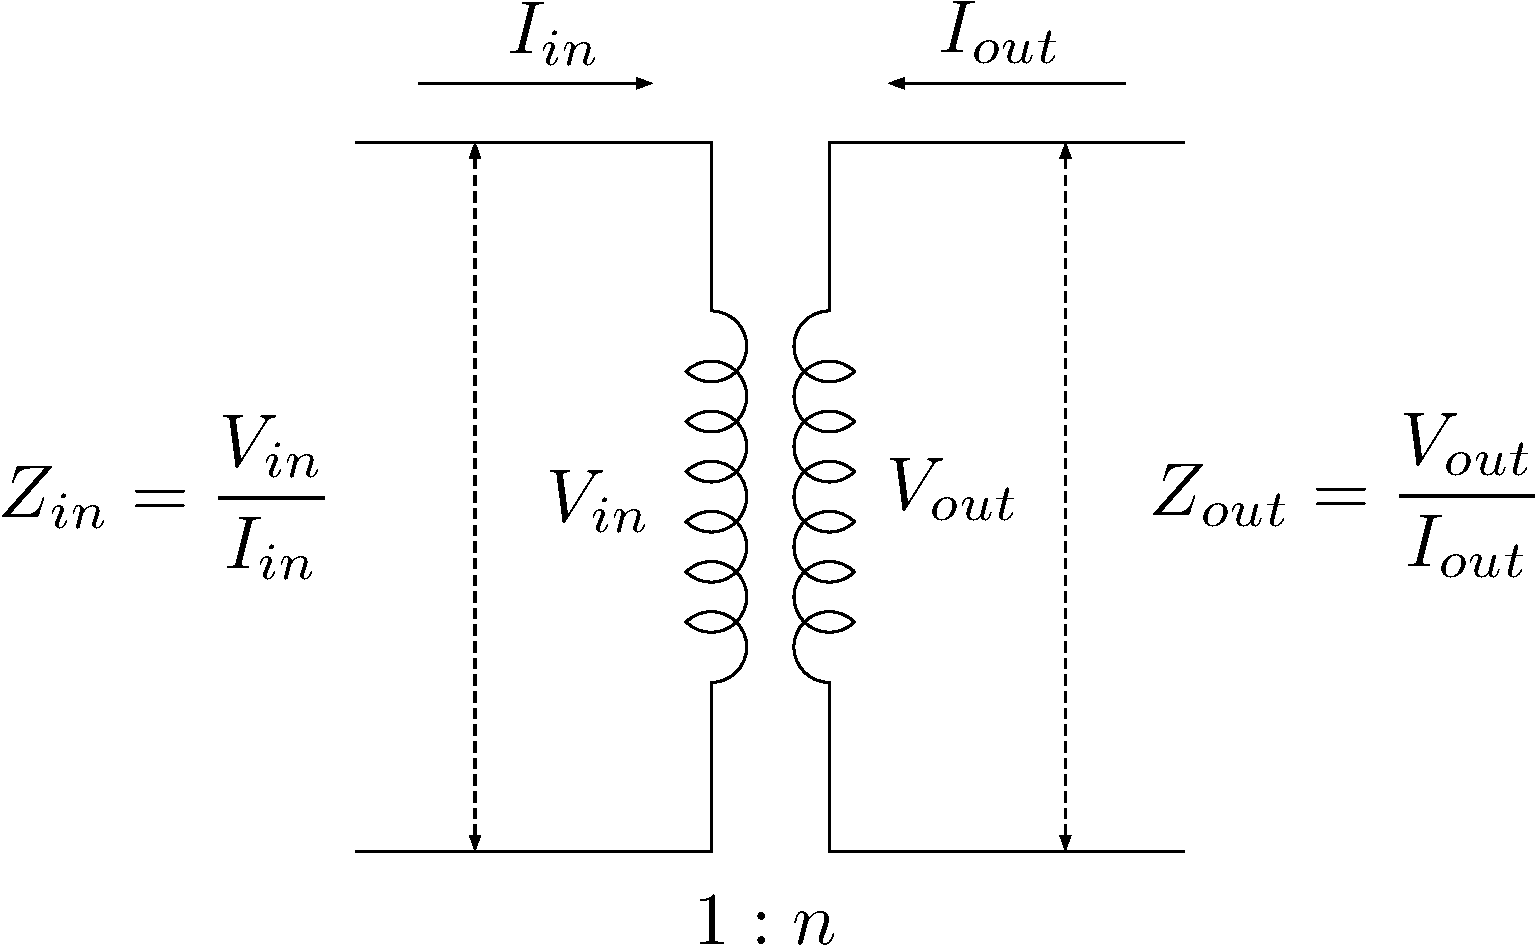
\includegraphics[width=12cm,clip]{figs/Ideal_Transformer.pdf}
        \caption{理想的なトランスによる入力カップラー.}
        \label{fig:Ideal_Trans}
    \end{center}
\end{figure}
%
\begin{equation}
    V_2 = N\cdot V_1, \; I_2 = \frac{1}{N}\cdot I_1
\end{equation}
%
したがって、
\begin{equation}
    Z_2 = n^2 \cdot Z_1
\end{equation}

\subsection{Available Power}
%
\begin{figure}[hbt]
    \begin{center}
        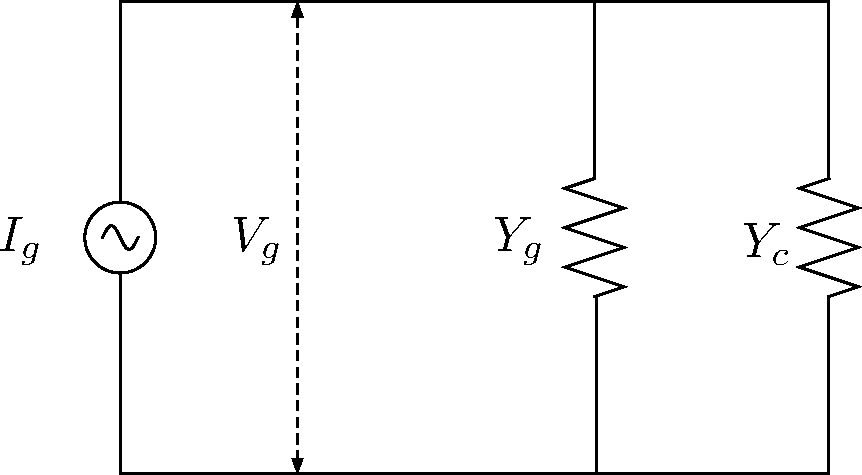
\includegraphics[width=12cm,clip]{figs/Available_Power.pdf}
        \caption{理想的なトランスによる入力カップラー.}
        \label{fig:Available_Power}
    \end{center}
\end{figure}
%
\begin{equation}
    P_{diss} = \frac{1}{2}Y_c V_g^2
\end{equation}
%
\begin{equation}
    V_g = \frac{I_g}{Y_L}=\frac{I_g}{Y_g+Y_c}
\end{equation}
%
\begin{equation}
    P_{diss} = \frac{1}{2}\frac{Y_c}{(Y_g+Y_c)^2}I_g^2
\end{equation}
%
\begin{equation}
    \begin{split}
        \frac{\partial P_{diss}}{\partial Y_c} &= \frac{1}{2}\frac{(Y_g + Y_c)^2 - 2Y_c(Y_g+Y_c)}{(Y_g+Y_c)^4} I_g^2 \\
        &= \frac{1}{2}\frac{Y_g-Y_c}{(Y_g+Y_c)^3} I_g^2
    \end{split}
\end{equation}
%
$\partial P_{diss}/\partial Y_c = 0$より、$Y_g = Y_c$の時、$P_{diss}$は最大になり
%
\begin{equation}
    P_{diss}^{max} = \frac{1}{8} Y_g I_g^2 = \frac{1}{8}\frac{R}{\beta}I_g^2 \equiv P_g
\end{equation}



\section{ビーム負荷付き空洞のRCL等価回路}

\begin{figure}[hbt]
    \begin{center}
        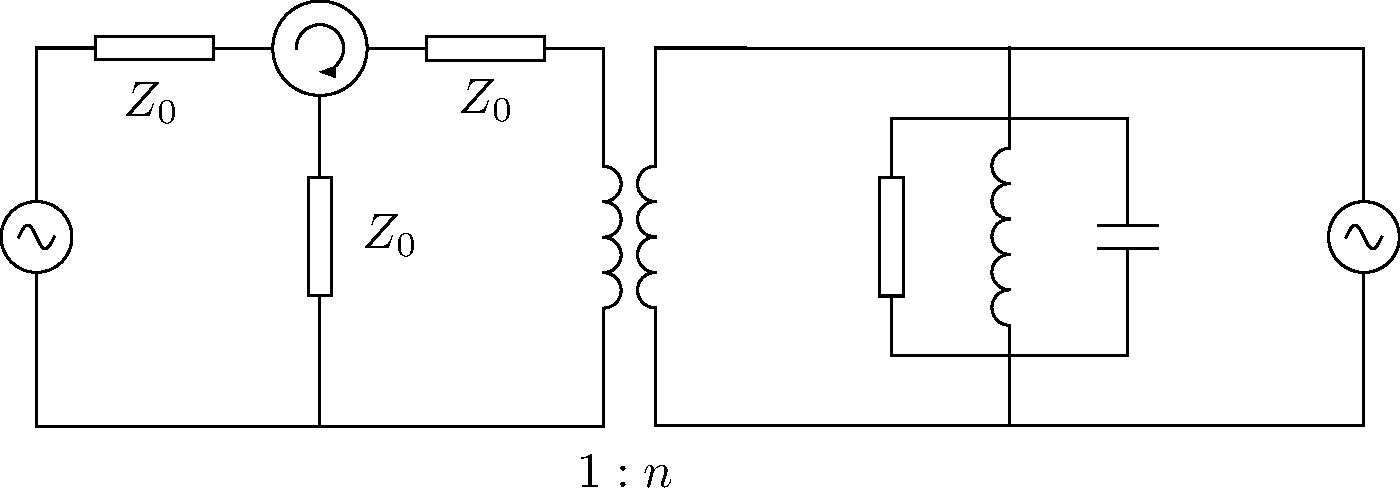
\includegraphics[width=12cm,clip]{figs/Cavity_Model.pdf}
        \caption{理想的なトランスによる入力カップラー.}
        \label{Cavity_Model}
    \end{center}
\end{figure}

\subsection{Cavity parameters}

\begin{figure}[hbt]
    \begin{center}
        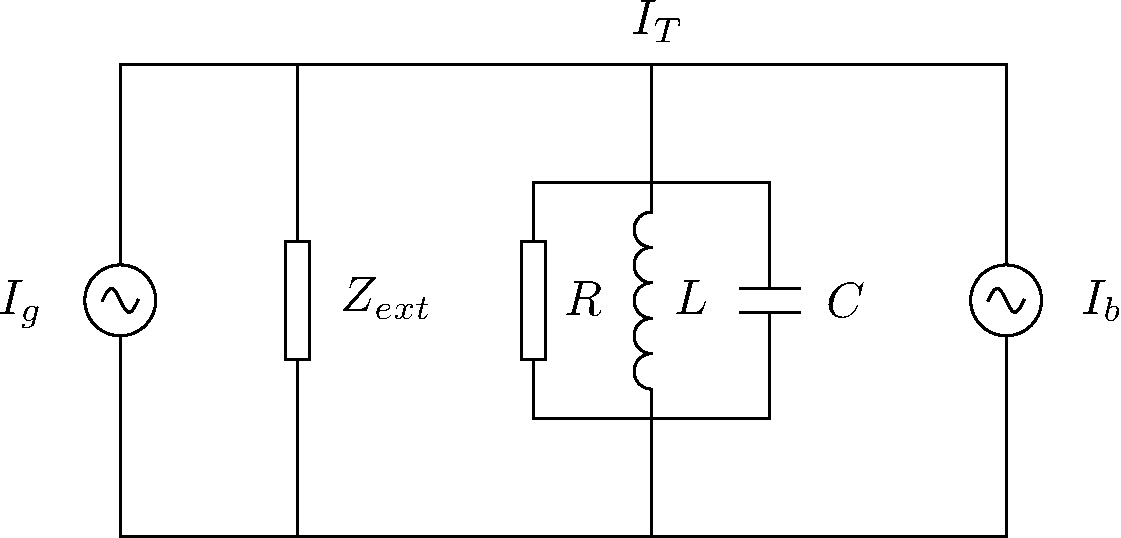
\includegraphics[width=12cm,clip]{figs/Equivalent_Circuit}
        \caption{等価回路}
        \label{Equivalent_Circuit}
    \end{center}
\end{figure}
%
\paragraph{共振周波数}
%
\begin{equation}
    \omega_0 = \frac{1}{L C}
\end{equation}
%
\paragraph{Quality factor}
%
\begin{equation}
    Q = 2\pi \frac{\mathrm{stored\;energy\;in\;cavity}}{\mathrm{dissipated \; energy\;per\;cycle}} = \frac{\omega_0 W}{P_{diss}}
\end{equation}
%
\paragraph{Unloaded quality factor}
%
\begin{equation}
    Q_0 = \omega_0 \frac{(1/2) C V^2}{V^2/(2R)} = \omega_0 R C
\end{equation}
%
\paragraph{External quality factor}
%
\begin{equation}
    Q_{ext} = 2\pi \frac{\mathrm{stored\;energy\;in\;cavity}}{\mathrm{dissipated \; energy\;in\;external\;devices\;per\;cycle}}
    = \frac{\omega_0 W}{P_{ext}}
\end{equation}
%
\paragraph{Loaded quality factor}
%
\begin{equation}
    Q_L = 2\pi \frac{\mathrm{stored\;energy\;in\;cavity}}{\mathrm{total \; energy\;per\;cycle}} = \frac{\omega_0 W}{P_{tot}}
\end{equation}
%
ここで、
%
\begin{equation}
    P_{tot} = P_{diss} + P_{ext}
\end{equation}
%
したがって、
%
\begin{equation}
    \frac{1}{Q_L} = \frac{1}{Q_0} + \frac{1}{Q_{ext}}
\end{equation}
%
\begin{equation}
    \frac{1}{R_L} = \frac{1}{R} + \frac{1}{Z_{ext}}
\end{equation}
%
\paragraph{Coupling factor \beta}
%
\begin{equation}
    \beta = \frac{P_{ext}}{P_{cav}} = \frac{Q_0}{Q_{ext}} = \frac{R}{Z_{ext}} = \frac{R}{n^2 Z_0}
\end{equation}
%
\begin{figure}[hbt]
    \begin{center}
        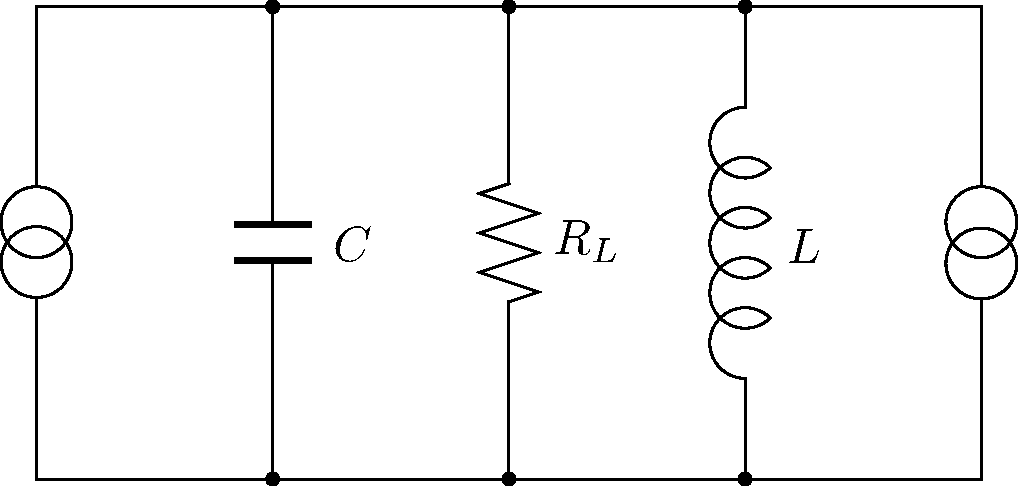
\includegraphics[width=12cm,clip]{figs/Equivalent_Circuit2}
        \caption{等価回路2}
        \label{Equivalent_Circuit2}
    \end{center}
\end{figure}
%
\begin{equation}
    \ddot{V}(t) + \frac{1}{R_L C}\dot{V}(t) + \frac{1}{L C} V(t) = \frac{1}{C} \dot{I}(t)
\end{equation}
%
\paragraph{Phasor}
\begin{equation}
    V(t) = \tilde{V}e^{j\omega_c t}, \; I(t) = \tilde{I}e^{j\omega_c t}
\end{equation}

\section{Cavity voltage}

\begin{equation}
    \left(\dv[2]{t}+\frac{\omega_c}{Q_L}\dv{t}+\omega_c^2\right)V_c(t)=\frac{\omega_c R_L}{Q_L}\dv{I_{tot}}{t}
\end{equation}

\section{Steady-state conditions}

\section{Analysis of small perturbations}

\begin{align}
    \delta V_c(t) = \frac{1}{2}\left\{V_c e^{-j\omega_g t}U(t)+ c.c\right\}
\end{align}


\section{Equations for cavity voltage}
\begin{equation}
    \begin{split}
        \vb*{V}_c(t) &= \tilde{V}(t)e^{j\omega_c t},\qquad \tilde{V}(t) = \hat{V}(1+a_v(t))e^{j(\phi_v(t)+\psi_v)} \\
        \vb*{I}_b(t) &= \tilde{I}_b(t) e^{j\omega_c t},\qquad \tilde{I}_b(t) = \hat{I}_b(1+a_b(t))e^{j(\phi_b(t)+\psi_b)} \\
        \vb*{I}_g(t) &= \tilde{I}_g(t) e^{j\omega_c t},\qquad \tilde{I}_g(t) = \hat{I}_g(1+a_g(t))e^{j(\phi_g(t)+\psi_g)} \\
        \vb*{I}_t(t) &= \vb*{I}_g(t) + \vb*{I}_b(t) = \tilde{I}_t(t) e^{j\omega_c t}
    \end{split}
\end{equation}
%
%
\begin{equation}
    \ddot{\vb*{V}_c}(t) + 2 \sigma \dot{\vb*{V}_c}(t) + \omega_0^2 \vb*{V}_c(t) = 2\sigma R \dot{\vb*{I}}_t(t)
\end{equation}
%
\clearpage

\chapter{Amplitude and phase modulation}
\section{Modulation Transfer Function}
%
振幅変調(AM)や位相変調(PM)された正弦波信号を伝達関数$H(s)$を持つシステムを介した場合、出力信号も一般に振幅変調と位相変調の両方を受けることになる。このようなシステムの完全な特性評価には、システムの伝達関数$H(s)$から導き出すことができる次の4つの異なる変調伝達関数(Modulation Transfer Function)を求める必要がある。(Fig.\ref{fig:MTF})
%
\begin{enumerate}
    \item 入力の振幅変調が出力の振幅を変調する伝達関数 : $G_{aa}(s)$
    \item 入力の位相変調が出力の位相を変調する伝達関数 : $G_{pp}(s)$
    \item 入力の振幅変調が出力の位相を変調する伝達関数 : $G_{ap}(s)$
    \item 入力の位相変量が出力の振幅を変調する伝達関数 : $G_{pa}(s)$
\end{enumerate}
%
\begin{figure}[hbt]
    \begin{center}
        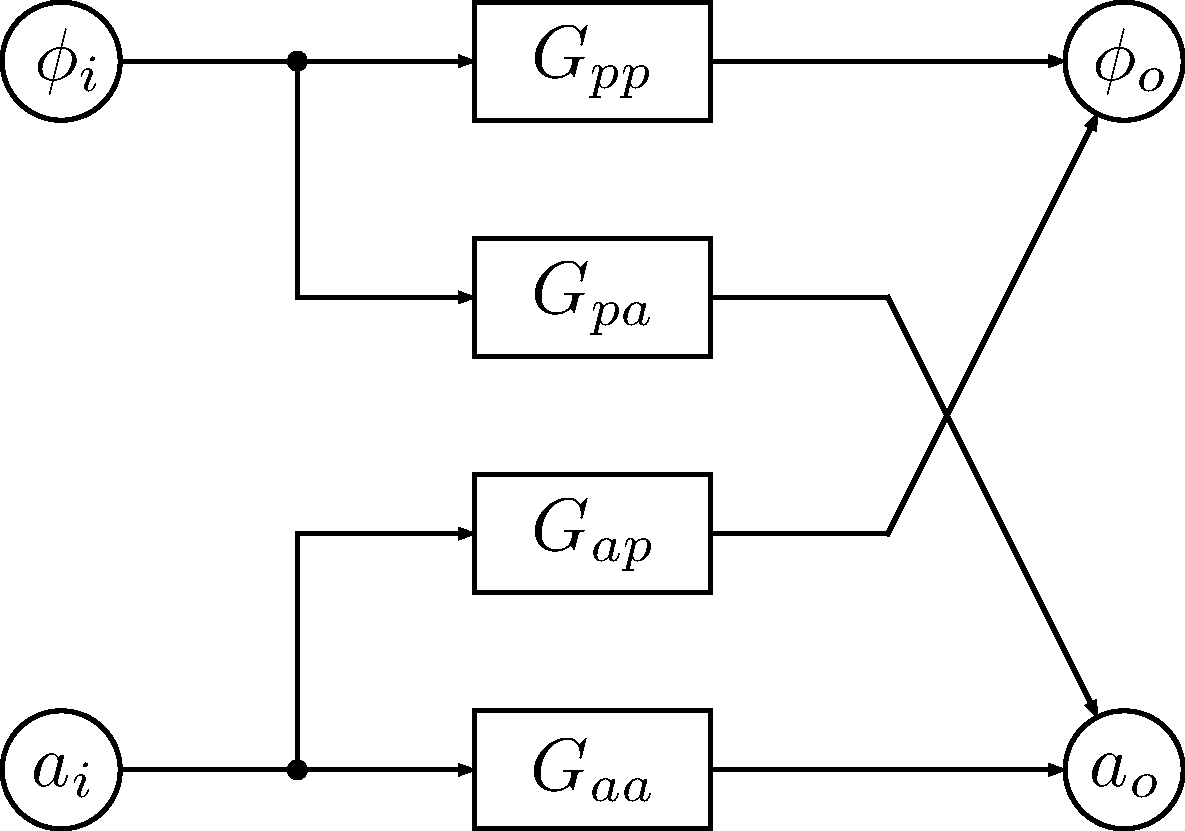
\includegraphics[width=8cm,clip]{figs/Mod_Trans_Func.pdf}
        \caption{Modulation Transfer Function.}
        \label{fig:MTF}
    \end{center}
\end{figure}
%
変調の振幅が十分小さい場合、変調の伝送は線形であり、次のようにして求めることができる。

最初に、入力信号の振幅のみが$a_i(t)$で変調された場合を考える。このとき、入力信号$x(t)$は次のようにあらわせる。
%
\begin{align}
    x(t) & = \Re\left \{\hat{X}(1 + a_i(t))e^{j\omega_c t}\right \}\notag   \\
         & = \hat{X}\left \{\cos\omega_c t + a_i(t) \cos\omega_c t\right \}
    \label{eq:in_am_sig1}
\end{align}
%
出力信号$y(t)$は$a_i(t)$によって振幅だけでなく位相も変調され、
%
\begin{equation}
    y(t) = \Re\left \{\hat{Y}(1 + a_{o,a}(t))e^{j(\omega_c t + \phi_0 + \phi_{o,a} (t))}\right \}
    \label{eq:out_am_sig1}
\end{equation}
%
と表すことができる。この時、変調伝達関数$G_{aa}(s),\;G_{ap}(s)$は、次のように定義される。
%
\begin{equation}
    G_{aa}(s) =  \frac{\hat{a}_{o, a}(s)}{\hat{a}_i(s)}, \quad G_{ap}(s) =  \frac{\hat{\phi}_{o, a}(s)}{\hat{a}_i(s)}
    \label{eq:am_tf}
\end{equation}
%
ここで、
%
\begin{align}
    \mathcal{L} [\cos\omega_c t]
     & = \frac{1}{2}\mathcal{L}[(e^{j\omega_c t}+e^{-j\omega_c t})]\notag                                                    \\
     & = \frac{1}{2}\left(\int_0^\infty e^{j\omega_c t} e^{-st} dt + \int_0^\infty e^{-j\omega_c t} e^{-st} dt \right)\notag \\
     & = \frac{1}{2}\left(\int_0^\infty e^{-(s-j\omega_c) t} dt + \int_0^\infty e^{-(s+j\omega_c) t} dt \right)\notag        \\
     & = \frac{1}{2}\left(\left[\frac{e^{-(s-j\omega_c) t}}{-(s-j\omega_c)}\right]_0^\infty +
    \left[\frac{e^{-(s+j\omega_c) t}}{-(s+j\omega_c)}\right]_0^\infty \right)\notag                                          \\
     & = \frac{1}{2}\left( \frac{1}{s-j\omega_c}+\frac{1}{s+j\omega_c}\right)
    = \frac{s}{s^2+\omega_c^2}
\end{align}
%
また、$\mathcal{L}\{a_i(t)\} = \hat{a}_i(s)$とすると、
%
\begin{align}
    \mathcal{L} [a_i(t)\cos\omega_c t]
     & = \frac{1}{2}\mathcal{L}[(a_i(t) e^{j\omega_c t}+a_i(t) e^{-j\omega_c t})]\notag                                                    \\
     & = \frac{1}{2}\left(\int_0^\infty a_i(t) e^{j\omega_c t} e^{-st} dt + \int_0^\infty a_i(t) e^{-j\omega_c t} e^{-st} dt \right)\notag \\
     & = \frac{1}{2}\left(\int_0^\infty a_i(t) e^{-(s-j\omega_c) t} dt + \int_0^\infty a_i(t) e^{-(s+j\omega_c) t} dt \right)\notag        \\
     & = \frac{1}{2}\{\hat{a}_i(s-j\omega_c) + \hat{a}_i(s+j\omega_c)\}
\end{align}
%
$X(s)=\mathcal{L}\{x(t)\}$とし、(\ref{eq:in_am_sig1})をラプラス変換すると、
%
\begin{equation}
    X(s) = \frac{\hat{X}}{2} \left \{\frac{2 s}{s^2 + \omega_c^2}
    + a_i(s - j\omega_c)+a_i(s+j\omega_c) \right \}
    \label{eq:lt_in_sig2}
\end{equation}
%
一方、出力信号$y(t)$は$a_o \ll 1,\; \phi_o \ll 1$の場合、以下のように近次できる。
%
\begin{align}
    y(t) & \simeq \Re{\hat{Y}(1+a_{o,a}(t))(1 + j\phi_{o,a}(t))e^{j(\omega_c t+\phi_o)}}\notag                        \\
         & = \Re{\hat{Y}(1 + a_{o,a}(t) + j\phi_{o,a}(t)
    + j\underset{0}{\uwave{a_{o,a}(t)\phi_{o,a}(t)}})e^{j(\omega_c t+\phi_0)}} \notag                                 \\
         & \simeq \Re{\hat{Y}(1+a_{o,a}(t)+j\phi_{o,a}(t))(\cos(\omega_c t + \phi_0)+j\sin(\omega_c + \phi_0))}\notag \\
         & = \hat{Y}\{\cos(\omega_c t+\phi_o)+a_o(t)\cos(\omega_c t+\phi_o) - \phi_o(t)\sin(\omega_c t + \phi_o)\}
    \label{eq:out_am_sig2}
\end{align}
%
ここで、
%
\begin{align}
    \mathcal{L} [\cos(\omega_c t + \phi_o)]
     & = \frac{1}{2}\mathcal{L}[(e^{j(\omega_c t+\phi_o)}+e^{-j(\omega_c t+\phi_o)})]\notag                                             \\
     & = \frac{1}{2}\left(\int_0^\infty e^{j(\omega_c t+\phi_o)} e^{-st} dt
    + \int_0^\infty e^{-j()\omega_c t+\phi_o)} e^{-st} dt \right)\notag                                                                 \\
     & = \frac{e^{j\phi_o}}{2}\int_0^\infty e^{-(s-j\omega_c) t} dt + \frac{e^{-j\phi_o}}{2}\int_0^\infty e^{-(s+j\omega_c) t} dt\notag \\
     & = \frac{e^{j\phi_o}}{2}\left[\frac{e^{-(s-j\omega_c) t}}{-(s-j\omega_c)}\right]_0^\infty
    +\frac{e^{-j\phi_o}}{2}\left[\frac{e^{-(s+j\omega_c) t}}{-(s+j\omega_c)}\right]_0^\infty\notag                                      \\
     & = \frac{1}{2}\left( \frac{e^{j\phi_o}}{s-j\omega_c}+\frac{e^{-j\phi_o}}{s+j\omega_c}\right)
    = \frac{\cos\phi_o s - \omega_c\sin\phi_o}{s^2+\omega_c^2}
\end{align}
%
また、$\mathcal{L}\{a_{o,a}(t)\} = \hat{a}_{o,a}(s),\; \mathcal{L}\{\phi_{o,a}(t)\} = \hat{\phi}_{o,a}(s)$とすると、
%
\begin{align}
    \mathcal{L} [a_{o,a}(t)\cos(\omega_c t+\phi_o)]
     & = \frac{1}{2}\mathcal{L}[(a_{o,a}(t) e^{j(\omega_c t+\phi_o)}+a_{o,a}(t) e^{-j(\omega_c t+\phi_o)})]\notag \\
     & = \frac{1}{2}\left(\int_0^\infty a_{o,a}(t) e^{j(\omega_c t+\phi_o)} e^{-st} dt
    + \int_0^\infty a_{o,a}(t) e^{-j(\omega_c t+\phi_o)} e^{-st} dt \right)\notag                                 \\
     & = \frac{e^{j\phi_o}}{2}\int_0^\infty a_{o,a}(t) e^{-(s-j\omega_c) t} dt
    + \frac{e^{-j\phi_o}}{2}\int_0^\infty a_{o,a}(t) e^{-(s+j\omega_c) t} dt\notag                                \\
     & = \frac{1}{2}\left\{e^{j\phi_o}\hat{a}_{o,a}(s-j\omega_c) + e^{-j\phi_o}\hat{a}_{o,a}(s+j\omega_c)\right\}
\end{align}
%
\begin{align}
    \mathcal{L} [\phi_{o,a}(t)\sin(\omega_c t+\phi_o)]
     & = \frac{1}{2j}\mathcal{L}[(\phi_{o,a}(t) e^{j(\omega_c t+\phi_o)} - \phi_{o,a}(t) e^{-j(\omega_c t+\phi_o)})]\notag \\
     & = \frac{1}{2j}\left(\int_0^\infty \phi_{o,a}(t) e^{j(\omega_c t+\phi_o)} e^{-st} dt
    - \int_0^\infty \phi_{o,a}(t) e^{-j(\omega_c t+\phi_o)} e^{-st} dt \right)\notag                                       \\
     & = \frac{e^{j\phi_o}}{2j}\int_0^\infty \phi_{o,a}(t) e^{-(s-j\omega_c) t} dt
    - \frac{e^{-j\phi_o}}{2j}\int_0^\infty \phi_{o,a}(t) e^{-(s+j\omega_c) t} dt\notag                                     \\
     & = -\frac{j}{2}\left\{e^{j\phi_o}\hat{\phi}_{o,a}(s-j\omega_c) - e^{-j\phi_o} \hat{\phi}_{o,a}(s+j\omega_c)\right\}
\end{align}
%
したがって、$Y(s)=\mathcal{L}\{y(t)\}$とし(\ref{eq:out_am_sig2})をラプラス変換すると、
%
\begin{multline}
    Y(s) = \frac{\hat{Y}}{2}\biggr [ \frac{2(\cos\phi_o s - \omega_c\sin\phi_o)}{s^2+\omega_c^2}
        + e^{j\phi_0}\hat{a}_{o, a}(s - j\omega_c) + e^{-j\phi_0}\hat{a}_{o, a}(s+j\omega_c) \\
        + j\left \{e^{j\phi_0}\hat{\phi}_{o,a}(s-j\omega_c) - e^{-j\phi_0}\hat{\phi}_{o,a}(s+j\omega_c) \right \} \biggl ]
    \label{eq:lt_out_am_sig2}
\end{multline}
%
ここで、(\ref{eq:am_tf})より(\ref{eq:lt_out_am_sig2})は
%
\begin{multline}
    Y(s) = \frac{\hat{Y}}{2}\biggr [ \frac{2(\cos\phi_o s - \omega_c\sin\phi_o)}{s^2+\omega_c^2}\\
    + e^{j\phi_0}G_{aa}(s-j\omega_c)\hat{a}_i(s - j\omega_c) + e^{-j\phi_0}G_{aa}(s+j\omega_c)\hat{a}_i(s+j\omega_c) \\
    + j\left \{e^{j\phi_0}G_{ap}(s-j\omega_c)\hat{a}_i(s-j\omega_c)
    - e^{-j\phi_0}G_{ap}(s+j\omega_c)\hat{a}_i(s+j\omega_c) \right \} \biggl ]\notag
\end{multline}
%
したがって、
%
\begin{multline}
    Y(s) = \frac{\hat{Y}}{2}\biggr [\frac{2(\cos\phi_0 s - \omega_c\sin\phi_0)}{s^2+\omega_c^2}
        + e^{j\phi_0}\{G_{aa}(s-j\omega_c)+j G_{ap}(s-j\omega_c)\}\hat{a}_i(s-j\omega_c) \\
        + e^{-j\phi_0}\{G_{aa}(s+j\omega_c)- j G_{ap}(s+j\omega_c)\}\hat{a}_i(s+j\omega_c)\biggl ]
    \label{eq:lt_out_am_sig3}
\end{multline}
%
ここで$Y(s) = H(s) X(s)$より、(\ref{eq:lt_in_sig2})は、
%
\begin{equation}
    Y(s) = \frac{\hat{X}H(s)}{2}\biggl [\frac{2 s}{(s^2+\omega_c^2} + \hat{a}_i(s - j\omega_c) + \hat{a}_i(s+j\omega_c)  \biggr ]
    \label{eq:lt_out_am_sig4}
\end{equation}
%
(\ref{eq:lt_out_am_sig3})と(\ref{eq:lt_out_am_sig4})で係数を比較すると、
%
\begin{equation}
    \hat{Y}(\cos\phi_0 s - \omega_c\sin\phi_0) = \hat{X}H(s) s
    \label{eq:coef1}
\end{equation}
%
\begin{equation}
    \begin{split}
        G_{aa}(s-j\omega_c) + j G_{ap}(s-j\omega_c) &= \frac{\hat{X}}{\hat{Y}}e^{-j\phi_0}H(s) \\
        G_{aa}(s+j\omega_c) - j G_{ap}(s+j\omega_c) &= \frac{\hat{X}}{\hat{Y}}e^{j\phi_0}H(s)
    \end{split}
    \label{eq:gaa_gap1}
\end{equation}
%
(\ref{eq:coef1})で、$s = \pm j\omega_c$の時を考えると、
%
\begin{equation}
    H(\pm j\omega_c) = \frac{\hat{Y}}{\hat{X}} e^{\pm j\phi_0}
    \label{eq:h_pm_jw}
\end{equation}
%
(\ref{eq:gaa_gap1})と(\ref{eq:h_pm_jw})より、
%
\begin{equation}
    \begin{split}
        G_{aa}(s-j\omega_c) + j G_{ap}(s-j\omega_c) &= \frac{H(s)}{H(j\omega_c)} \\
        G_{aa}(s+j\omega_c) - j G_{ap}(s+j\omega_c) &= \frac{H(s)}{H(-j\omega_c)}
    \end{split}
    \label{eq:gaa_gap2}
\end{equation}
%
以上より、入力の振幅変調に関する変調伝達関数$G_{aa}(s),\;G_{ap}(s)$は、
%
\begin{equation}
    \begin{split}
        G_{aa}(s) &= \frac{1}{2}\left\{\frac{H(s+j\omega_c)}{H(j\omega_c)} + \frac{H(s-j\omega_c)}{H(-j\omega_c)}\right\} = G_s(s)\\
        G_{ap}(s) &= \frac{-j}{2}\left\{\frac{H(s+j\omega_c)}{H(j\omega_c)} - \frac{H(s-j\omega_c)}{H(-j\omega_c)}\right\} = G_c(s)
    \end{split}
\end{equation}

今度は、入力信号の位相のみが$\phi_i(t)$で変調された信号を考えると、
%
\begin{equation}
    x(t) = \Re\{\hat{X} e^{j(\omega_ct + \phi_i(t))}\}
    \label{eq:in_pm_sig1}
\end{equation}
%
出力信号は先程と同様に考えると、
%
\begin{equation}
    y(t) = \Re\{\hat{Y}(1+a_{o, p}(t))e^{j(\omega_c t + \phi_0 + \phi_{o, p}(t))}\}
    \label{eq:out_pm_sig1}
\end{equation}
%
入力の位相変調に関する変調伝達関数$G_{pp}(s),\;G_{pa}(s)$は、
%
\begin{equation}
    G_{pp}(s) = \frac{\hat{\phi}_{o, p}(s)}{\hat{\phi}_i(s)}, \quad G_{pa}(s) = \frac{\hat{a}_{o, p}(s)}{\hat{\phi}_i(s)}
    \label{eq:pm_tf}
\end{equation}
%
(\ref{eq:in_pm_sig1})は、$\phi_i(t) \ll 1$の時、
%
\begin{equation}
    \begin{split}
        x(t) &= \Re\{\hat{X} e^{j(\omega_c t + \phi_i(t))}\} \\
        &\simeq \Re\{\hat{X}(1+j\phi_i(t)) e^{j\omega_c t}\} \\
        &= \hat{X} (\cos\omega_c t - \phi_i(t)\sin\omega_c t ) \\
        \label{eq:in_pm_sig2}
    \end{split}
\end{equation}
%
(\ref{eq:in_pm_sig2})をラプラス変換すると、
%
\begin{equation}
    X(s) = \hat{X}\left [\frac{s}{s^2+\omega_c^2}
        + j \left \{\hat{\phi}_i(s - j\omega_c) - \hat{\phi}_i(s+j\omega_c)\right \} \right ]
    \label{eq:lt_in_pm_sig2}
\end{equation}
%
(\ref{eq:lt_out_am_sig2})と同様にして(\ref{eq:out_pm_sig1})もラプラス変換すると、
%
\begin{multline}
    Y(s) = \frac{\hat{Y}}{2}\biggr [\frac{2(\cos\phi_0 s - \omega_c\sin\phi_0)}{s^2+\omega_c^2}
    + e^{j\hat{\phi}_0}a_{o, p}(s - j\omega_c) + e^{-j\phi_0}\hat{a}_{o, p}(s+j\omega_c) \\
    + j\left \{e^{j\phi_0}\hat{\phi}_{o,p}(s-j\omega_c) - e^{-j\phi_0}\hat{\phi}_{o,p}(s+j\omega_c) \right \} \biggl ]
    \label{eq:lt_out_pm_sig2}
\end{multline}
%
同様に(\ref{eq:lt_out_pm_sig2})は
%
\begin{multline}
    Y(s) = \frac{\hat{Y}}{2}\biggr [\frac{2(\cos\phi_0 s - \omega_c\sin\phi_0)}{s^2+\omega_c^2}
        + e^{j\phi_0}\{G_{pa}(s-j\omega_c)+j G_{pp}(s-j\omega_c)\}\hat{\phi}_i(s-j\omega_c) \\
        + e^{-j\phi_0}\{G_{pa}(s+j\omega_c)- j G_{pp}(s+j\omega_c)\}\hat{\phi}_i(s+j\omega_c)\biggl ]
    \label{eq:lt_out_pm_sig3}
\end{multline}
%
ここで$Y(s) = H(s) X(s)$より、
%
\begin{equation}
    Y(s) = \frac{\hat{X}H(s)}{2} \biggl [\frac{2 s}{s^2+\omega_c^2}
        + j \left \{\hat{\phi}_i(s - j\omega_c) - \hat{\phi}_i(s+j\omega_c)\right \}  \biggr ]
    \label{eq:lt_out_pm_sig4}
\end{equation}
%
(\ref{eq:lt_out_pm_sig3})と(\ref{eq:lt_out_pm_sig4})で係数を比較すし、(\ref{eq:h_pm_jw})を使うと、
%
\begin{equation}
    \begin{split}
        G_{pa}(s-j\omega_c) + j G_{pp}(s-j\omega_c) &= j \frac{H(s)}{H(j\omega_c)} \\
        G_{pa}(s+j\omega_c) - j G_{pp}(s+j\omega_c) &= -j \frac{H(s)}{H(-j\omega_c)}
    \end{split}
\end{equation}
%
したがって、
%
\begin{equation}
    \begin{split}
        G_{pa}(s) + j G_{pp}(s) &= j \frac{H(s+j\omega_c)}{H(j\omega_c)} \\
        G_{pa}(s) - j G_{pp}(s) &= -j \frac{H(s-j\omega_c)}{H(-j\omega_c)}
    \end{split}
\end{equation}
%
以上の結果から、変調伝達関数は以下の様になる。
%
\begin{equation}
    \begin{aligned}
        G_{aa}(s) & = G_{pp}(s)
                  & = \frac{1}{2}\left\{\frac{H(s+j\omega_c)}{H(j\omega_c)} + \frac{H(s-j\omega_c)}{H(-j\omega_c)}\right\} & = G_s(s) \\
        G_{ap}(s) & = -G_{pa}(s)
                  & = \frac{j}{2}\left\{\frac{H(s+j\omega_c)}{H(j\omega_c)} - \frac{H(s-j\omega_c)}{H(-j\omega_c)}\right\} & = G_c(s)
    \end{aligned}
\end{equation}
%
\subsection{空洞共振器への適用}
%
\begin{equation}
    Z(s) = \frac{2\sigma R_s}{s^2+2\sigma s + \omega_r^2}
\end{equation}
%
\begin{align}
    G_{aa}(s) & = G_{pp} = \frac{\sigma^2(1+\tan^2\phi_z)+\sigma s}{s^2+2\sigma s + \sigma^2(1+\tan^2\phi_z)} \\
    G_{pa}(s) & = - G_{ap} = \frac{\sigma\tan\phi_z s}{s^2+2\sigma s + \sigma^2(1+\tan^2\phi_z)}
\end{align}
%



\chapter{Robinson instability}

\appendix
\chapter{周波数伝達関数}
\section{部分分数展開を用いたラプラス逆変換の計算}
一般に、有理関数で表された伝達関数$G(s)$は、
%
\begin{equation}
    G(s)=K\frac{(s+z_1)(s+z_2)\dots(s+z_m)}{(s+p_1)(s+p_2)\dots(s+p_n)}
\end{equation}
%

入力を、$u(t)=e^{j\omega t}$とすると、ラプラス変換は、次式で与えられる。
%
\begin{equation}
    U(s)= \mathcal{L}[u(t)]=\mathcal{L}[e^{j\omega t}]=\frac{1}{s-j\omega}
\end{equation}
%
したがって、出力$Y(s)=\mathcal{L}[y(t)]$は、次のように部分分数展開できる。
%
\begin{equation}
    \begin{split}
        Y(s) &= G(s)U(s) = \frac{k(s-z_1)(s-z_2)\dots(s-z_m)}{(s-p_1)(s-p_2)\dots(s-p_n)}\frac{1}{s-j\omega} \\
        &= \frac{k_1}{s-p_1}+\frac{k_2}{s-p_2}+\dots+\frac{k_n}{s-p_n}+\frac{a}{s-j\omega}\notag
    \end{split}
\end{equation}
%
ただし、
%
\begin{equation}
    \begin{split}
        k_i &= \lim_{s \to p_i}(s-p_i)G(s)\frac{s}{s-j\omega} \\
        a &=\lim_{s \to j\omega}(s-j\omega)G(s)\frac{1}{s-j\omega} =\lim_{s \to j\omega}G(s)\cdot 1=G(j\omega)
    \end{split}
\end{equation}
%
したがって、出力は$Y(s)$を逆ラプラス変換して次式で求められる。
%
\begin{equation}
    y(t)=k_1 e^{p_1 t}+k_2 e^{p_2 t}+ \dots + k_n e^{p_n t} + a e^{j\omega t}
\end{equation}
%
極の実部は負であるから、定常状態では次式で与えられる。
%
\begin{equation}
    y(t) = a e^{j\omega t} = G(j\omega) e^{j\omega t}
\end{equation}
%
\chapter{ラプラス変換}
%
\begin{align}
    \mathcal{L} [\cos\omega_c t]
     & = \frac{1}{2}\mathcal{L}[(e^{j\omega_c t}+e^{-j\omega_c t})]\notag                                                    \\
     & = \frac{1}{2}\left(\int_0^\infty e^{j\omega_c t} e^{-st} dt + \int_0^\infty e^{-j\omega_c t} e^{-st} dt \right)\notag \\
     & = \frac{1}{2}\left(\int_0^\infty e^{-(s-j\omega_c) t} dt + \int_0^\infty e^{-(s+j\omega_c) t} dt \right)\notag        \\
     & = \frac{1}{2}\left(\left[\frac{e^{-(s-j\omega_c) t}}{-(s-j\omega_c)}\right]_0^\infty +
    \left[\frac{e^{-(s+j\omega_c) t}}{-(s+j\omega_c)}\right]_0^\infty \right)\notag                                          \\
     & = \frac{1}{2}\left( \frac{1}{s-j\omega_c}+\frac{1}{s+j\omega_c}\right)
    = \frac{s}{s^2+\omega_c^2}
    \label{eq:lt_cos}
\end{align}
%
\begin{align}
    \mathcal{L} [\cos(\omega_c t + \phi_o)]
     & = \frac{1}{2}\mathcal{L}[(e^{j(\omega_c t+\phi_o)}+e^{-j(\omega_c t+\phi_o)})]\notag                                             \\
     & = \frac{1}{2}\left(\int_0^\infty e^{j(\omega_c t+\phi_o)} e^{-st} dt
    + \int_0^\infty e^{-j()\omega_c t+\phi_o)} e^{-st} dt \right)\notag                                                                 \\
     & = \frac{e^{j\phi_o}}{2}\int_0^\infty e^{-(s-j\omega_c) t} dt + \frac{e^{-j\phi_o}}{2}\int_0^\infty e^{-(s+j\omega_c) t} dt\notag \\
     & = \frac{e^{j\phi_o}}{2}\left[\frac{e^{-(s-j\omega_c) t}}{-(s-j\omega_c)}\right]_0^\infty
    +\frac{e^{-j\phi_o}}{2}\left[\frac{e^{-(s+j\omega_c) t}}{-(s+j\omega_c)}\right]_0^\infty\notag                                      \\
     & = \frac{1}{2}\left( \frac{e^{j\phi_o}}{s-j\omega_c}+\frac{e^{-j\phi_o}}{s+j\omega_c}\right)
    = \frac{\cos\phi_o s - \omega_c\sin\phi_o}{s^2+\omega_c^2}
    \label{eq:lt_cos_phi0}
\end{align}
%
$\mathcal{L}\{a_i(t)\} = \hat{a}_i(s)$とすると、
%
\begin{align}
    \mathcal{L} [a_i(t)\cos\omega_c t]
     & = \frac{1}{2}\mathcal{L}[(a_i(t) e^{j\omega_c t}+a_i(t) e^{-j\omega_c t})]\notag                                                    \\
     & = \frac{1}{2}\left(\int_0^\infty a_i(t) e^{j\omega_c t} e^{-st} dt + \int_0^\infty a_i(t) e^{-j\omega_c t} e^{-st} dt \right)\notag \\
     & = \frac{1}{2}\left(\int_0^\infty a_i(t) e^{-(s-j\omega_c) t} dt + \int_0^\infty a_i(t) e^{-(s+j\omega_c) t} dt \right)\notag        \\
     & = \frac{1}{2}\{\hat{a}_i(s-j\omega_c) + \hat{a}_i(s+j\omega_c)\}
    \label{eq:lt_ai_cos}
\end{align}
%
$\mathcal{L}\{a_{o,a}(t)\} = \hat{a}_{o,a}(s),\; \mathcal{L}\{\phi_{o,a}(t)\} = \hat{\phi}_{o,a}(s)$とすると、
%
\begin{align}
    \mathcal{L} [a_{o,a}(t)\cos(\omega_c t+\phi_o)]
     & = \frac{1}{2}\mathcal{L}[(a_{o,a}(t) e^{j(\omega_c t+\phi_o)}+a_{o,a}(t) e^{-j(\omega_c t+\phi_o)})]\notag \\
     & = \frac{1}{2}\left(\int_0^\infty a_{o,a}(t) e^{j(\omega_c t+\phi_o)} e^{-st} dt
    + \int_0^\infty a_{o,a}(t) e^{-j(\omega_c t+\phi_o)} e^{-st} dt \right)\notag                                 \\
     & = \frac{e^{j\phi_o}}{2}\int_0^\infty a_{o,a}(t) e^{-(s-j\omega_c) t} dt
    + \frac{e^{-j\phi_o}}{2}\int_0^\infty a_{o,a}(t) e^{-(s+j\omega_c) t} dt\notag                                \\
     & = \frac{1}{2}\left\{e^{j\phi_o}\hat{a}_{o,a}(s-j\omega_c) + e^{-j\phi_o}\hat{a}_{o,a}(s+j\omega_c)\right\}
\end{align}
%
\begin{align}
    \mathcal{L} [\phi_{o,a}(t)\sin(\omega_c t+\phi_o)]
     & = \frac{1}{2j}\mathcal{L}[(\phi_{o,a}(t) e^{j(\omega_c t+\phi_o)} - \phi_{o,a}(t) e^{-j(\omega_c t+\phi_o)})]\notag \\
     & = \frac{1}{2j}\left(\int_0^\infty \phi_{o,a}(t) e^{j(\omega_c t+\phi_o)} e^{-st} dt
    - \int_0^\infty \phi_{o,a}(t) e^{-j(\omega_c t+\phi_o)} e^{-st} dt \right)\notag                                       \\
     & = \frac{e^{j\phi_o}}{2j}\int_0^\infty \phi_{o,a}(t) e^{-(s-j\omega_c) t} dt
    - \frac{e^{-j\phi_o}}{2j}\int_0^\infty \phi_{o,a}(t) e^{-(s+j\omega_c) t} dt\notag                                     \\
     & = -\frac{j}{2}\left\{e^{j\phi_o}\hat{\phi}_{o,a}(s-j\omega_c) - e^{-j\phi_o} \hat{\phi}_{o,a}(s+j\omega_c)\right\}
\end{align}




\section{Pedersen Model}
\subsection{空洞を介した位相、振幅、チューニング伝送}

位相および振幅が変調された正弦波信号は次のように表せる。




位相および振幅変調された正弦波信号を送信する場合:


$a_i(t)$で振幅変調され、$\phi(t)$で位相変調された角振動数$\omega_c$の正弦波信号は、次のように表される。
%
\begin{equation}
    x(t) = \Re{A_i(1+a_i(t))e^{j(\omega_c t+\phi_i(t))}}
    \label{eq:in_sig1}
\end{equation}
%
$a_i \ll 1,\; \phi_i \ll 1$の場合、(\ref{eq:in_sig1})は
%
\begin{align}
    x(t) & \simeq \Re{A_i(1 + a_i(t))(1 + j\phi_i(t))e^{j\omega_c t}}                                \notag   \\
         & = \Re{A_i(1 + a_i(t) + j\phi_i(t) + j\underset{0}{\uwave{a_i(t)\phi_i(t)}})e^{j\omega_c t}} \notag \\
         & \simeq \Re{A_i(1 + a_i(t) + j\phi_i(t))e^{j\omega_c t}}\notag                                      \\
         & = \Re{A_i(1 + a_i(t) + j\phi_i(t))(\cos\omega_c t + j\sin\omega_c t)} \notag                       \\
         & = A_i(\cos\omega_c t + a_i(t)\cos\omega_c t - \phi(t)\sin\omega_c t)
    \label{eq:in_sig2}
\end{align}
%
ここで、
%
\begin{align}
    \mathcal{L} [\cos\omega_c t]
     & = \frac{1}{2}\mathcal{L}[(e^{j\omega_c t}+e^{-j\omega_c t})]\notag                                                    \\
     & = \frac{1}{2}\left(\int_0^\infty e^{j\omega_c t} e^{-st} dt + \int_0^\infty e^{-j\omega_c t} e^{-st} dt \right)\notag \\
     & = \frac{1}{2}\left(\int_0^\infty e^{-(s-j\omega_c) t} dt + \int_0^\infty e^{-(s+j\omega_c) t} dt \right)\notag        \\
     & = \frac{1}{2}\left(\left[\frac{e^{-(s-j\omega_c) t}}{-(s-j\omega_c)}\right]_0^\infty +
    \left[\frac{e^{-(s+j\omega_c) t}}{-(s+j\omega_c)}\right]_0^\infty \right)\notag                                          \\
     & = \frac{1}{2}\left( \frac{1}{s-j\omega_c}+\frac{1}{s+j\omega_c}\right)
    = \frac{s}{s^2+\omega_c^2}
\end{align}
%
また、$\mathcal{L}\{a_i(t)\} = a_i(s),\; \mathcal{L}\{\phi_i(t)\} = \phi_i(s)$とすると、
%
\begin{align}
    \mathcal{L} [a_i(t)\cos\omega_c t]
     & = \frac{1}{2}\mathcal{L}[(a_i(t) e^{j\omega_c t}+a_i(t) e^{-j\omega_c t})]\notag                                                    \\
     & = \frac{1}{2}\left(\int_0^\infty a_i(t) e^{j\omega_c t} e^{-st} dt + \int_0^\infty a_i(t) e^{-j\omega_c t} e^{-st} dt \right)\notag \\
     & = \frac{1}{2}\left(\int_0^\infty a_i(t) e^{-(s-j\omega_c) t} dt + \int_0^\infty a_i(t) e^{-(s+j\omega_c) t} dt \right)\notag        \\
     & = \frac{a_i(s-j\omega_c) + a_i(s+j\omega_c)}{2}
\end{align}
%
\begin{align}
    \mathcal{L} [\phi_i(t)\sin\omega_c t]
     & = \frac{1}{2j}\mathcal{L}[(\phi_i(t) e^{j\omega_c t} - \phi_i(t) e^{-j\omega_c t})]\notag \\
     & = \frac{1}{2j}\left(\int_0^\infty \phi_i(t) e^{j\omega_c t} e^{-st} dt -
    \int_0^\infty \phi_i(t) e^{-j\omega_c t} e^{-st} dt \right)\notag                            \\
     & = \frac{1}{2j}\left(\int_0^\infty \phi_i(t) e^{-(s-j\omega_c) t} dt -
    \int_0^\infty \phi_i(t) e^{-(s+j\omega_c) t} dt \right)\notag                                \\
     & = \frac{\phi_i(s-j\omega_c) - \phi_i(s+j\omega_c)}{2j}
\end{align}
%
以上より、$X(s) = \mathcal{L}\{x(t)\}$とし、(\ref{eq:in_sig2})をラプラス変換すると、
%
\begin{equation}
    X(s) = \frac{A_i}{2}\left\{ \frac{2s}{s^2+\omega_c^2}
    + a_i(s-j\omega_c) + j\phi_i(s-j\omega_c)
    + a_i(s+j\omega_c) - j\phi_i(s+j\omega_c) \right\}
\end{equation}

伝達関数$H(s)$を介して、出力される信号$y(t)$は一般的に振幅と位相の両方は変調され、次の様に表せる。
%
\begin{equation}
    y(t) = \Re{A_o(1+a_o(t))e^{j(\omega_c t+\phi_z + \phi_o(t))}}
    \label{eq:out_sig1}
\end{equation}
%
$a_o \ll 1,\; \phi_o \ll 1$の場合、(\ref{eq:out_sig1})は
%
\begin{align}
    y(t) & \simeq \Re{A_o(1+a_o(t))(1 + j\phi_o(t))e^{j(\omega_c t+\phi_z)}}\notag                                     \\
         & = \Re{A_i(1 + a_o(t) + j\phi_o(t) + j\underset{0}{\uwave{a_o(t)\phi_o(t)}})e^{j(\omega_c t+\phi_z)}} \notag \\
         & \simeq \Re{A_o(1+a_o(t)+j\phi_o(t))(\cos(\omega_c t + \phi_z)+j\sin(\omega_c + \phi_z))}\notag              \\
         & = A_o(\cos(\omega_c t+\phi_z)+a_o(t)\cos(\omega_c t+\phi_z) - \phi_o(t)\sin(\omega_c t + \phi_z))
    \label{eq:out_sig2}
\end{align}
%
ここで、
%
\begin{align}
    \mathcal{L} [\cos(\omega_c t + \phi_z)]
     & = \frac{1}{2}\mathcal{L}[(e^{j(\omega_c t+\phi_z)}+e^{-j(\omega_c t+\phi_z)})]\notag                                             \\
     & = \frac{1}{2}\left(\int_0^\infty e^{j(\omega_c t+\phi_z)} e^{-st} dt
    + \int_0^\infty e^{-j()\omega_c t+\phi_z)} e^{-st} dt \right)\notag                                                                 \\
     & = \frac{e^{j\phi_z}}{2}\int_0^\infty e^{-(s-j\omega_c) t} dt + \frac{e^{-j\phi_z}}{2}\int_0^\infty e^{-(s+j\omega_c) t} dt\notag \\
     & = \frac{e^{j\phi_z}}{2}\left[\frac{e^{-(s-j\omega_c) t}}{-(s-j\omega_c)}\right]_0^\infty
    +\frac{e^{-j\phi_z}}{2}\left[\frac{e^{-(s+j\omega_c) t}}{-(s+j\omega_c)}\right]_0^\infty\notag                                      \\
     & = \frac{1}{2}\left( \frac{e^{j\phi_z}}{s-j\omega_c}+\frac{e^{-j\phi_z}}{s+j\omega_c}\right)
    = \frac{\cos\phi_z s - \omega_c\sin\phi_z}{s^2+\omega_c^2}
\end{align}
%
また、$\mathcal{L}\{a_o(t)\} = a_o(s),\; \mathcal{L}\{\phi_o(t)\} = \phi_o(s)$とすると、
%
\begin{align}
    \mathcal{L} [a_o(t)\cos(\omega_c t+\phi_z)]
     & = \frac{1}{2}\mathcal{L}[(a_o(t) e^{j(\omega_c t+\phi_z)}+a_o(t) e^{-j(\omega_c t+\phi_z)})]\notag \\
     & = \frac{1}{2}\left(\int_0^\infty a_o(t) e^{j(\omega_c t+\phi_z)} e^{-st} dt
    + \int_0^\infty a_o(t) e^{-j(\omega_c t+\phi_z)} e^{-st} dt \right)\notag                             \\
     & = \frac{e^{j\phi_z}}{2}\int_0^\infty a_o(t) e^{-(s-j\omega_c) t} dt
    + \frac{e^{-j\phi_z}}{2}\int_0^\infty a_o(t) e^{-(s+j\omega_c) t} dt\notag                            \\
     & = \frac{e^{j\phi_z}}{2}a_o(s-j\omega_c) + \frac{e^{-j\phi_z}}{2} a_o(s+j\omega_c)
\end{align}
%
\begin{align}
    \mathcal{L} [\phi_o(t)\sin(\omega_c t+\phi_z)]
     & = \frac{1}{2j}\mathcal{L}[(\phi_o(t) e^{j(\omega_c t+\phi_z)} - \phi_o(t) e^{-j(\omega_c t+\phi_z)})]\notag \\
     & = \frac{1}{2j}\left(\int_0^\infty \phi_o(t) e^{j(\omega_c t+\phi_z)} e^{-st} dt
    - \int_0^\infty \phi_o(t) e^{-j(\omega_c t+\phi_z)} e^{-st} dt \right)\notag                                   \\
     & = \frac{e^{j\phi_z}}{2j}\int_0^\infty \phi_o(t) e^{-(s-j\omega_c) t} dt
    - \frac{e^{-j\phi_z}}{2j}\int_0^\infty \phi_o(t) e^{-(s+j\omega_c) t} dt\notag                                 \\
     & = \frac{e^{j\phi_z}}{2j}\phi_o(s-j\omega_c) - \frac{e^{-j\phi_z}}{2j} \phi_o(s+j\omega_c)
\end{align}
%
以上より、$Y(s) = \mathcal{L}\{y(t)\}$とし、(\ref{eq:out_sig2})をラプラス変換すると、
%
\begin{multline}
    Y(s) = A_o\biggr [\frac{\cos\phi_z s - \omega_c\sin\phi_z}{s^2+\omega_c^2}
        +  \frac{e^{j\phi_z}}{2}\{a_o(s-j\omega_c) + j \phi_o(s-j\omega_c)\}\\
        + \frac{e^{-j\phi_z}}{2}\{a_o(s+j\omega_c) + j \phi_o(s+j\omega_c)\}\biggl ]
    \label{eq:lt_out_sig2}
\end{multline}
%
ここで、
%
\begin{equation}
    \left\{
    \begin{aligned}
        a_o(s)    & = G_{aa}(s) a_i(s) + G_{pa}(s)\phi_i(s) \\
        \phi_o(s) & = G_{ap}(s) a_i(s) + G_{pp}(s)\phi_i(s)
        \label{eq:tf}
    \end{aligned}
    \right.
\end{equation}
%
より、(\ref{eq:tf})を(\ref{eq:lt_out_sig2})に代入すると、
%
\begin{multline}
    Y(s) = \frac{A_o}{2}\biggr [\frac{2(\cos\phi_z s - \omega_c\sin\phi_z)}{s^2+\omega_c^2}\\
        + e^{j\phi_z}\{(G_{aa}(s-j\omega_c) +j G_{ap}(s-j\omega_c)) a_i(s-j\omega_c)\\
        + (G_{pa}(s-j\omega_c) +j G_{pp}(s-j\omega_c))\} \phi_i(s-j\omega_c)\\
        + e^{-j\phi_z}\{(G_{aa}(s+j\omega_c) -j G_{ap}(s+j\omega_c)) a_i(s+j\omega_c)\\
        + (G_{pa}(s+j\omega_c) -j G_{pp}(s+j\omega_c))\} \phi_i(s-+j\omega_c) \biggl ]
    \label{eq:lt_out_sig3}
\end{multline}
%
ここで$Y(s) = H(s) X(s)$より、
%
\begin{equation}
    Y(s) = \frac{A_i H(s)}{2}\left\{ \frac{2s}{s^2+\omega_c^2}
    + a_i(s-j\omega_c) + j\phi_i(s-j\omega_c)
    + a_i(s+j\omega_c) - j\phi_i(s+j\omega_c) \right\}
    \label{eq:lt_out_sig4}
\end{equation}
%
(\ref{eq:lt_out_sig3})と(\ref{eq:lt_out_sig4})で係数を比較すると、


\chapter{加速空洞の等価回路}
\section{RLC並列共振回路の微分方程式}
%
\begin{figure}[hbt]
    \begin{center}
        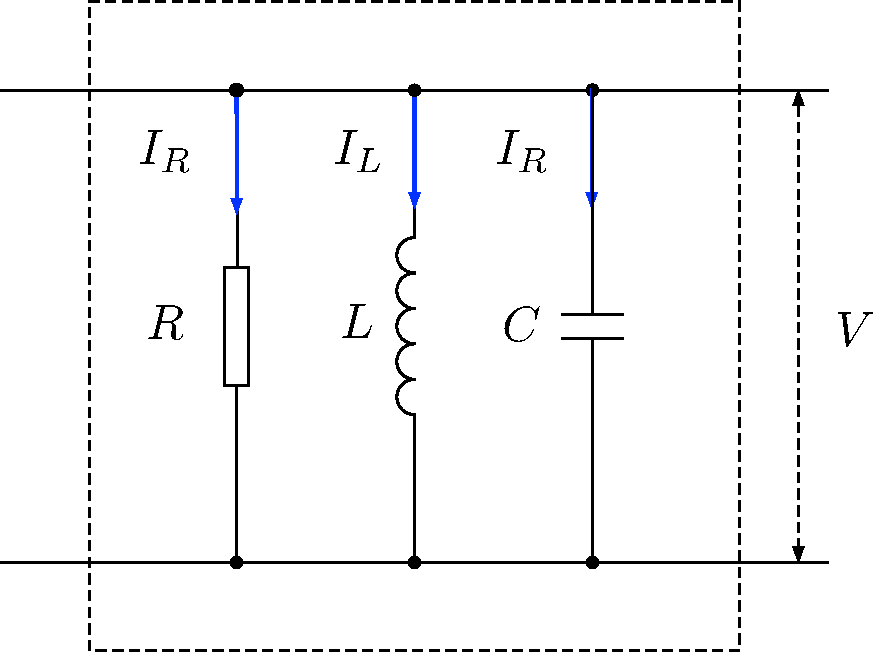
\includegraphics[width=12cm,clip]{figs/RLC_Model.pdf}
        \caption{Cavity RLC Model}
        \label{fig:RLC}
    \end{center}
\end{figure}
%
\begin{equation}
    \begin{split}
        I(t) &= I_R(t) + I_L(t) + I_C(t) \\
        I_R(t) &= \frac{V(t)}{R}, \; I_L(t) = \frac{1}{L}\int V(t) dt, \; I_c(t) = C\frac{dV(t)}{dt}
    \end{split}
\end{equation}
%
したがって、
%
\begin{equation}
    \frac{V(t)}{R} + \frac{1}{L}\int V(t) dt + C\frac{dV(t)}{dt} = I(t)
\end{equation}
%
両辺を時間$t$で微分すると、
%
\begin{equation}
    \frac{\dot{V}(t)}{R} + \frac{V(t)}{L}+ C \ddot{V(t)} = \dot{I(t)}
\end{equation}
%
\begin{equation}
    \ddot{V}(t) + \frac{1}{CR}\dot{V}(t) + \frac{1}{LC} V(t) = \frac{1}{C}\dot{I}(t)
\end{equation}
%
\begin{equation}
    \omega_0^2 = \frac{1}{LC}, \qquad \sigma = \frac{R}{2}\sqrt{\frac{C}{L}} = \frac{\omega_0}{2Q_L}
\end{equation}
%
\begin{equation}
    \ddot{V}(t) + 2 \sigma \dot{V}(t) + \omega_0^2 V(t) = 2\sigma R \dot{I}(t)
\end{equation}
%
\begin{thebibliography}{9}
    \bibitem{Pedersen}
    F. Pedersen, Beam Loading Effects in the CERN PS Booster, IEEE Trans. Nucl. Sci. 22, 3, June 1975.
    \bibitem{Ninomiya}
    S. Ninomiya, Beam Loading Effect on RF System in Proton Synchrotrons, KEK Report 89-18 (1989).
    \bibitem{llrf}
    S. Simrock, Z. Geng, Low-Level Radio Frequency Systems, Springer (2022)
    \bibitem{Schilcher}
    T. Schilcher Vector sum control of pulsed accelerating fields in Lorentz force detuned superconducting cavities (1998).
    \bibitem{Wilson}
    P. B. Wilson, High energy electron linacs; application to storage ring RF systems and linear colliders (1987)
\end{thebibliography}
%
%
\end{document}